\apendice{Documentación técnica de programación}

\section{Introducción}
En este apartado de los anexos voy a comentar:
\begin{itemize}
	\item \textbf{Estructura de directorios:} estructura de directorios con la que se ha trabajado en \textit{GitHub}.
	\item \textbf{Manual del programador:} manual en el que se explican los pasos que se ha de realizar para seguir desarrollando el proyecto.
	\item \textbf{Compilación, instalación y ejecución del proyecto:} explicación de los pasos a realizar para la instalación y ejecución del proyecto.
	\item \textbf{Pruebas del sistema:} pruebas realizas en el desarrollo del proyecto.
\end{itemize}
\section{Estructura de directorios}
La estructura de directorios que he seguido para la realización de este proyecto es la misma que se puede ver en el repositorio en \textit{GitHub}, \url{https://github.com/Josemi/AVC-TFG}. Esta estructura, en primer nivel, se puede ver como:
\dirtree{%
	.1 /.
	.2 app.
	.2 doc.
	.2 server.
}

En la carpeta \textit{app}, nos encontramos con el código de las 3 aplicaciones desarrolladas con \textit{AndroidStudio} en el proyecto. Éstas son \textit{Aplicacion} que es la aplicación prototipo de grabación de audios, \textit{AplicacionGSAudios} que es la aplicación para la recogida de datos y \textit{AplicacionFinal} que es la aplicación de interpretación AVC. Además, nos encontramos con una carpeta llamada \textit{apks}, donde se encuentran las \textit{apks} de las últimas versiones de cada aplicación. El árbol que cuelga de la carpeta \textit{app} se puede ver a continuación:

\dirtree{%
	.1 app.
	.2 Aplicacion.
	.2 AplicacionGSAudios.
	.2 Aplicacion.
	.2 apks.
}

En la carpeta \textit{doc} nos encontramos con la estructura de documentación del proyecto, la cual se puede ver en el siguiente árbol:
\dirtree{%
	.1 doc.
	.2 Diseño.
	.3 AplicaciónFinal.
	.4 DiagramasDeClase.
	.4 DiagramasSecuencia.
	.4 Errores.
	.4 Interfaces.
	.4 Pruebas.
	.3 AplicaciónGSAudios.
	.3 Servidor.
	.3 Casos de uso.
	.2 javadoc.
	.3 AplicacionFinal.
	.3 AplicacionGSAudios.
	.3 Aplicacion.
	.2 Vídeos.
	.2 Final.
	.2 Manuales de usuario.
	.3 Manual AVC.
	.3 Manual-Presentación-RecogidaDeDatos.
	.3 ManualUsuarioPrototipo.
	.2 Presentación28mayo.
	.2 Símbolos.
}

Como se puede observar, de la carpeta \textit{doc} cuelgan muchos elementos. Entre ellos están los orientados al diseño de la aplicación en la carpeta \textit{Diseño}, a los manuales de usuario en la carpeta \textit{Manuales de usuario} o por ejemplo a la estructura para generar la documentación final en \LaTeX{} en la carpeta \textit{Final}.

Dentro de la carpeta \textit{javadoc}, podemos encontrar la documentación de las 3 aplicaciones realizadas. En la carpeta \textit{Vídeos} es donde podemos encontrar los distintos vídeos explicativos que he creado para enseñar las aplicaciones.

Cabe destacar que en la carpeta \textit{Símbolos} nos encontramos con los pictogramas de \textit{ARASAAC}~\cite{arasaac}, los cuales hemos modificado para utilizarlos en la aplicación de interpretación final.

Por último en la carpeta \textit{server} nos encontramos con la siguiente estructura:
\dirtree{%
	.1 server.
	.2 prueba.
	.2 final.
}

En la carpeta \textit{prueba}, encontramos con la primera prueba que realicé para usar \textit{Flask}, y en la carpeta \textit{final} nos encontramos con la estructura del servidor final ya comentada en el apartado~\ref{server}
\section{Manual del programador}
En este apartado se va a comentar que se tendría que hacer para, a partir del software actual, realizar mejoras. Para este apartado se ha decidido no explicar la aplicación prototipo, ya que el resto de aplicaciones son mejoras a partir de ésta. Además, se tiene en cuenta que se dispone de la estructura del proyecto tras haber hecho un \textit{clone} del repositorio en \textit{GitHub}.
\subsection{Aplicación para la recogida de datos}
El código de esta aplicación se encuentra en el directorio \textit{/app/AplicaciónGSAudios}. Para poder modificar el código de esta aplicación tenemos que abrir \textit{AndroidStudio}, pulsar \textit{File} y después \textit{Open\ldots}, aquí se nos abrirá un diálogo en el cual podremos elegir la aplicación, \textit{AndroidStudio} se encarga de buscar las aplicaciones y de mostrarlas para poder elegir la aplicación, como se puede ver en la figura~\ref{fig:andstu}.

\begin{figure}
	\centering
	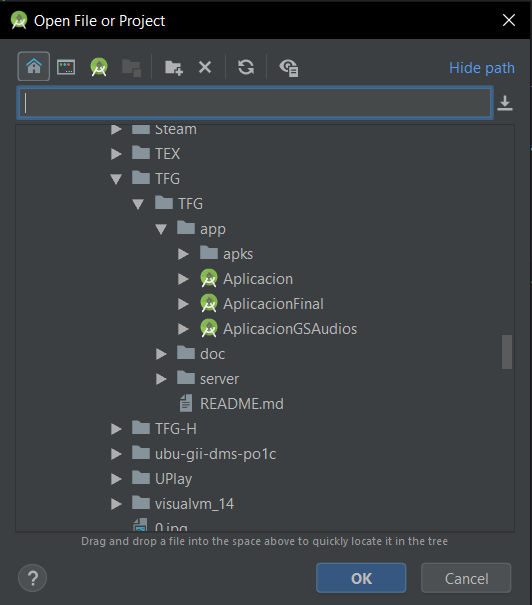
\includegraphics[scale=0.5]{andstu}
	\caption{Selección de fichero o proyecto en \textit{AndroidStudio}.}
	\label{fig:andstu}
\end{figure}

Una vez hayamos seleccionado y abierto el proyecto tendremos en \textit{AndroidStudio} una vista de la estructura del proyecto. Tras procesar y cargar el proyecto, que según el tamaño de este puede durar un rato, \textit{AndroidStudio} nos organiza las carpetas en dos, \textit{app} y \textit{Gradle Scripts}, como se puede ver en la ~\ref{fig:estappgd}.

\begin{figure}
	\centering
	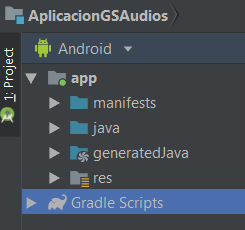
\includegraphics[scale=0.7]{estappgd}
	\caption{Estructura de ficheros generada por \textit{AndroidStudio}.}
	\label{fig:estappgd}
\end{figure}

En la carpeta \textit{app} nos encontramos con la lógica y las interfaces de las pantallas, mientras que en la carpeta \textit{Gradle Scripts} nos encontramos algunas configuraciones importantes del proyecto, como los \textit{imports} de las librerías externas o la API mínima de desarrollo.

Dentro de la carpeta de \textit{app} nos encontramos con la siguiente estructura:
\dirtree{%
	.1 app.
	.2 manifest.
	.2 java.
	.2 generatedJava.
	.2 res.
}

En la carpeta \textit{manifest} nos encontramos con uno de los ficheros más importantes del desarrollo en \textit{Android}. Es en él donde se encuentran los permisos que tiene la aplicación, para el acceso a Internet, para la grabación de audios\ldots En la carpeta \textit{java} nos encontramos con la lógica de la aplicación y con los test para probar esta lógica. Por último, en la carpeta \textit{res} nos encontramos con la estructura que nos permite administrar y utilizar los archivos como imágenes, sonidos y sobre todo los \textit{layouts} que son las interfaces de las pantallas.

Una de las posibles modificaciones que se podrían querer hacer a esta aplicación sería añadir algún paciente al cual poder grabar, para ello tenemos que acceder a la carpeta \textit{/res/values} y en concreto al archivo \textit{strings.xml}, donde podemos encontrar el \textit{array} con los pacientes, el cual se carga al principio de la aplicación en el \textit{spinner} de selección de paciente.

\subsection{Aplicación para la interpretación}
Para abrir el proyecto con esta aplicación tenemos que seguir los mismos pasos que en la aplicación anterior, pero a la hora de abrir el proyecto tenemos que seleccionar \textit{AplicaciónFinal}.

La estructura de este proyecto es similar a la anterior, pero más completa, ya que en este nos encontramos con más imágenes, sonidos e incluso ficheros donde se definen las formas y los colores de los botones, todo ello en la carpeta \textit{res}.
\subsection{Servidor}
La estructura del servidor ha sido explicada en el apartado~\ref{server}. Si se quiere modificar algún apartado de su lógica tendríamos que modificar el fichero \textit{apiserver.py} donde se encuentra el servidor \textit{Flask}.

Una de las posibles modificaciones que se pueden hacer sobre el servidor es, como en la aplicación de generación de datos, añadir un paciente al sistema. Para ello tenemos que abrir el fichero \textit{paciente.csv} y añadir el nombre del paciente nuevo. Además, tenemos que crear el fichero \textit{csv}, puede ser vacío, en la carpeta \textit{Opciones} con el mismo nombre que se ha puesto en el fichero \textit{pacientes.csv}. Por último, si se quiere que la interpretación no se haga de forma aleatoria tenemos que añadir los modelos de clasificación correspondientes en la carpeta \textit{Modelos}, además de modificar el flujo del método \textit{clasifica} del servidor.

Aun así, si metemos un nuevo paciente en el fichero \textit{pacientes.csv} y no se crean los ficheros necesarios, una vez queramos acceder desde la aplicación para la interpretación nos devolverá el error correspondiente que nos dirá que documentos nos faltan en el servidor.
\section{Compilación, instalación y ejecución del proyecto}
En este apartado se va a comentar la instalación y ejecución del servidor, ya que la instalación y ejecución de las aplicaciones se van a comentar en el apartado de \textit{Manual de usuario}.

\subsection{Requisitos}
\begin{itemize}
	\item Tener una tarjeta de red que nos permita a partir del programa \textit{noWifi} crear una red, con esa tarjeta como \textit{router}.
	\item Tener instalado \textit{Python 3} actualizado, en concreto la ejecución se va a mostrar con \textit{Anaconda}.
	\item Tener instaladas las librerías de \textit{sklearn}, \textit{numpy}, \textit{flask}, \textit{base64}, \textit{csv}, \textit{datetime}, \textit{os}, \textit{librosa}, \textit{random}, \textit{glob}, \textit{pydub} y \textit{matplotlib}, si no se tiene instalada algunas de estas librerías tendríamos que instalarlas en su última versión.
\end{itemize}

\subsection{Instalación}
El único software que hay que instalar, a parte de \textit{Python} y las librerías, son las aplicaciones que ya se menciona su instalación en los manuales de usuario.

\subsection{Ejecución}
Para la ejecución lo primero tenemos que hacer es desactivar el \textit{FireWall} de sistema operativo \textit{Windows}, después tenemos que abrir el programa \textit{noWifi} y crear nuestra propia red cumplimentando el \textit{SSID}, con el nombre que queremos que tenga nuestra red, y \textit{Password} con la contraseña que queremos que tenga la red. Una vez hemos cumplimentado eso, tenemos que pulsar el \textit{checkbox} llamado \textit{Access Point} para iniciar la red, como se ve en la figura~\ref{fig:nw}.

\begin{figure}
	\centering
	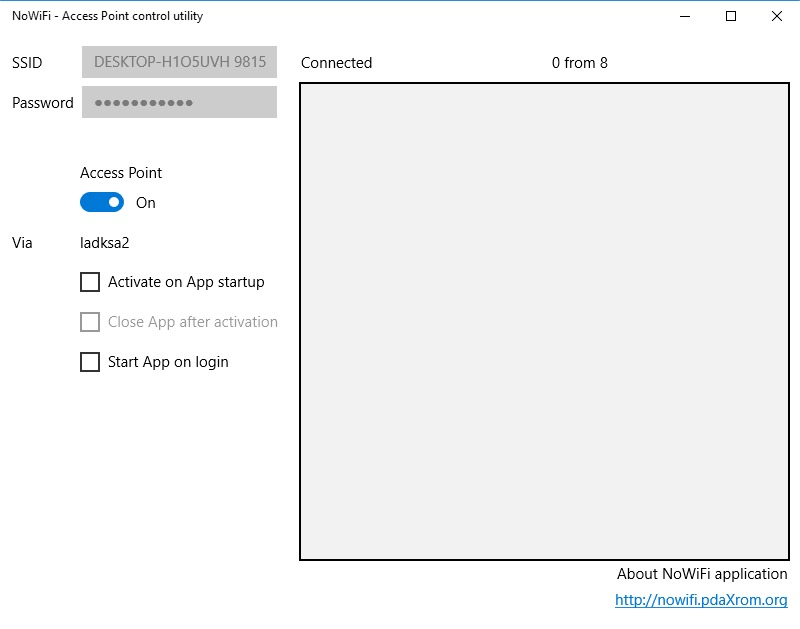
\includegraphics[width=\textwidth]{nw}
	\caption{Interfaz de \textit{noWifi}.}
	\label{fig:nw}
\end{figure}

Es a esta red a la cual nos tenemos que conectar desde el dispositivo que quiere ejecutar la aplicación para la interpretación, \textit{AVC}. Como se puede ver en la figura~\ref{fig:nw}, hay un apartado llamado \textit{Connected} donde podemos observar los dispositivos conectados a nuestra red.

Después de crear y configurar nuestra red, tenemos que abrir \textit{Anaconda Prompt} para desplegar el servidor. Para ello lo primero que tenemos que hacer en esta consola es movernos a las carpeta \textit{/server/final} del servidor, como se ve en la figura~\ref{fig:cd}.

\begin{figure}
	\centering
	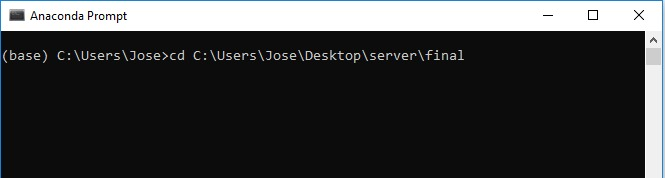
\includegraphics[width=\textwidth]{cd}
	\caption{Comando cd a la carpeta \textit{/server/final}.}
	\label{fig:cd}
\end{figure}

Tras movernos a la carpeta donde se encuentra el código del servidor \textit{Flask}, solo tenemos que ejecutar el fichero \textit{Python} con el comando \textit{python apiserver.py}, como se puede ver en la figura~\ref{fig:py}.

\begin{figure}
	\centering
	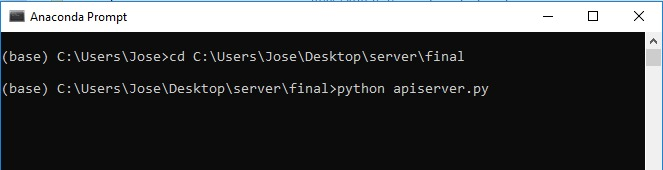
\includegraphics[width=\textwidth]{py}
	\caption{Comando \textit{Python} para desplegar el servidor.}
	\label{fig:py}
\end{figure}

Una vez ejecutado el comando empezará a desplegarse el servidor en \textit{Flask}. Esto puede llevar un tiempo debido a que \textit{Flask}, como nos dice cada vez que hacemos una ejecución, no es un \textit{framework} para desarrollar servidores de producción, sino para desarrollar pruebas de estos. Después de que el servidor se haya cargado (sabemos que está cargado porque no pone la dirección \textit{IP} sobre la que se está ejecutando) podremos ver las distintas llamas al servidor junto con la dirección \textit{IP} de la llamada, el día y la hora, el método del servidor al cual se ha llamado y por último el código de respuesta que se ha devuelto. Todo esto se puede ver en la figura~\ref{fig:res}.

\begin{figure}
	\centering
	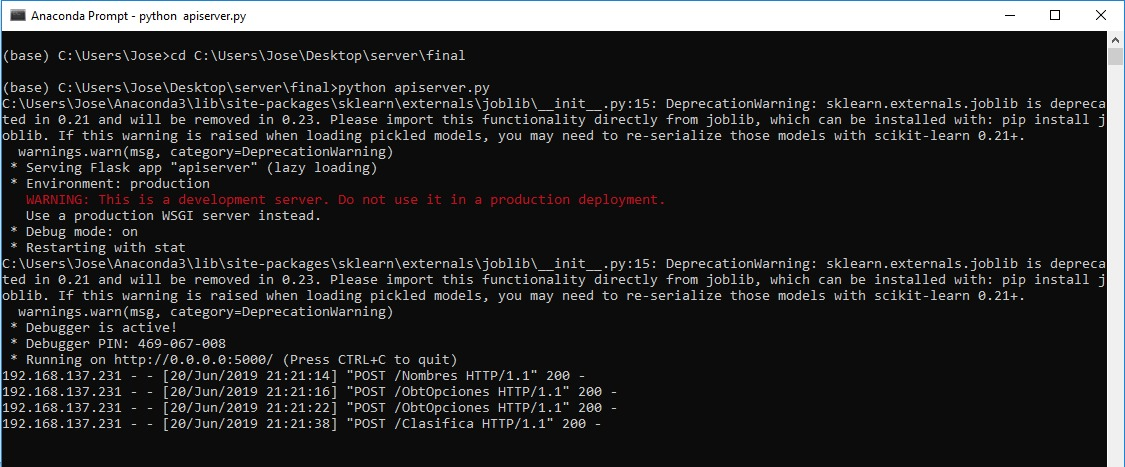
\includegraphics[width=\textwidth]{res}
	\caption{Consola del servidor en ejecución.}
	\label{fig:res}
\end{figure}

Los \textit{DeprecationWarnings} que se ven en la ejecución son debido a la librería que ha decidido usar el investigador colaborador, Sergio Chico, para almacenar los modelos.
\section{Pruebas del sistema}
Las pruebas en un proyecto software son esenciales, ya que nos permiten probar las funcionalidades y el comportamiento del software desarrollado. Su finalidad es detectar fallos, es decir, una conjunto de pruebas tienen éxito cuando descubren algún \textit{bug} o mal comportamiento en el software.

En este proyecto se han hecho pruebas sobre la aplicación más importante, la aplicación de interpretación. Debido a la necesidad de tener la aplicación para la recogida de datos lo antes posible, para poder trabajar con el mayor número de éstos, no se pudieron realizar test. Aun así la aplicación se probó en diversos dispositivos para encontrar los \textit{bugs} más graves y significativos.

Se han elaborado distintos tipos de pruebas en la aplicación de interpretación y por ende en el servidor. Éstas se pueden clasificar en dos tipos:
\begin{itemize}
	\item \textbf{Unitarias:} prueban la que la lógica y la creación de las clases es correcta.
	\item \textbf{Integración:} prueban que la colaboración entre las distintas clases es correcta.
	\item \textbf{Estrés:} prueban el comportamiento de la aplicación en situaciones complicadas de mucho trabajo.
\end{itemize}

En total se han realizado de 82 test entre test unitarios y de integración, en los que he utilizado diferentes herramientas orientadas a los test como son \textit{Espresso} y \textit{JUnit}. El resultado de los 82 test se puede ver en la figura~\ref{fig:test}.
\begin{figure}
	\centering
	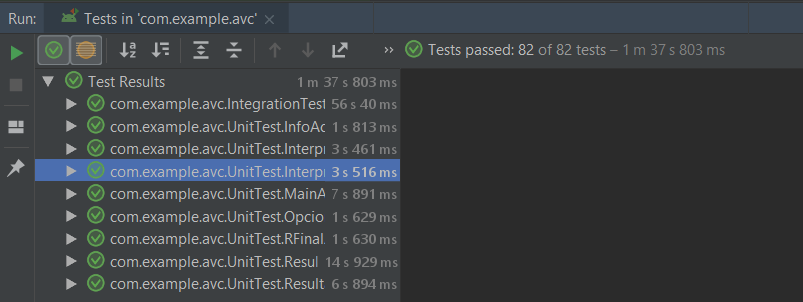
\includegraphics[width=\textwidth]{test}
	\caption{Salida de los test unitarios y de integración.}
	\label{fig:test}
\end{figure}

Además, he realizado pruebas de test con la herramienta \textit{MonkeyTest}, que permite en su ejecución probar las aplicaciones en situaciones de estrés, con muchas pulsaciones, todas ellas aleatorias para poder probar todos los apartados de la aplicación. Debido a la velocidad de esta prueba, solo se  ha usado en la versión de la aplicación de interpretación sin conexión al servidor.

Para ejecutar el \textit{MonkeyTest} tenemos que hacer los siguientes pasos en el mismo orden:
\begin{itemize}
	\item Abrir una consola \textit{cmd}.
	\item Movernos a la carpeta \textit{C:\textbackslash Users\textbackslash Usuario\textbackslash AppData\textbackslash Local\textbackslash Android\textbackslash Sdk\textbackslash platform-tools}
	\item Ejecutar el comando \textit{adb -e(simulador)/-d(dispositivo conectado) shell monkey -p [package de la app] -v(para obtener más información de cómo ha ido la ejecución) [Número de eventos aleatorios]}.
\end{itemize}

Un ejemplo del comando de ejecución sería, \textit{adb -d shell monkey -p com.example.avc -v 1000 > test.txt}, en el cual decimos que lo queremos ejecutar en un dispositivo conectado, que el paquete donde se encuentra nuestra aplicación es \textit{com.example.avc}, que queremos obtener información adicional sobre la ejecución, que queremos que haga 1.000 eventos aleatorios y por último que la salida por consola la desvíe al fichero \textit{test.txt}.

Tras la ejecución podremos ver en el fichero el conjunto de acciones que ha ido haciendo, así como su resultado final, es decir, si la ejecución se ha detenido o no.